% Options for packages loaded elsewhere
\PassOptionsToPackage{unicode}{hyperref}
\PassOptionsToPackage{hyphens}{url}
%
\documentclass[
  ignorenonframetext,
  aspectratio=169]{beamer}
\usepackage{pgfpages}
\setbeamertemplate{caption}[numbered]
\setbeamertemplate{caption label separator}{: }
\setbeamercolor{caption name}{fg=normal text.fg}
\beamertemplatenavigationsymbolsempty
% Prevent slide breaks in the middle of a paragraph
\widowpenalties 1 10000
\raggedbottom
\setbeamertemplate{part page}{
  \centering
  \begin{beamercolorbox}[sep=16pt,center]{part title}
    \usebeamerfont{part title}\insertpart\par
  \end{beamercolorbox}
}
\setbeamertemplate{section page}{
  \centering
  \begin{beamercolorbox}[sep=12pt,center]{part title}
    \usebeamerfont{section title}\insertsection\par
  \end{beamercolorbox}
}
\setbeamertemplate{subsection page}{
  \centering
  \begin{beamercolorbox}[sep=8pt,center]{part title}
    \usebeamerfont{subsection title}\insertsubsection\par
  \end{beamercolorbox}
}
\AtBeginPart{
  \frame{\partpage}
}
\AtBeginSection{
  \ifbibliography
  \else
    \frame{\sectionpage}
  \fi
}
\AtBeginSubsection{
  \frame{\subsectionpage}
}
\usepackage{amsmath,amssymb}
\usepackage{lmodern}
\usepackage{iftex}
\ifPDFTeX
  \usepackage[T1]{fontenc}
  \usepackage[utf8]{inputenc}
  \usepackage{textcomp} % provide euro and other symbols
\else % if luatex or xetex
  \usepackage{unicode-math}
  \defaultfontfeatures{Scale=MatchLowercase}
  \defaultfontfeatures[\rmfamily]{Ligatures=TeX,Scale=1}
  \setmainfont[]{IPAPMincho}
\fi
\usefonttheme{serif} % use mainfont rather than sansfont for slide text
% Use upquote if available, for straight quotes in verbatim environments
\IfFileExists{upquote.sty}{\usepackage{upquote}}{}
\IfFileExists{microtype.sty}{% use microtype if available
  \usepackage[]{microtype}
  \UseMicrotypeSet[protrusion]{basicmath} % disable protrusion for tt fonts
}{}
\makeatletter
\@ifundefined{KOMAClassName}{% if non-KOMA class
  \IfFileExists{parskip.sty}{%
    \usepackage{parskip}
  }{% else
    \setlength{\parindent}{0pt}
    \setlength{\parskip}{6pt plus 2pt minus 1pt}}
}{% if KOMA class
  \KOMAoptions{parskip=half}}
\makeatother
\usepackage{xcolor}
\newif\ifbibliography
\usepackage{color}
\usepackage{fancyvrb}
\newcommand{\VerbBar}{|}
\newcommand{\VERB}{\Verb[commandchars=\\\{\}]}
\DefineVerbatimEnvironment{Highlighting}{Verbatim}{commandchars=\\\{\}}
% Add ',fontsize=\small' for more characters per line
\usepackage{framed}
\definecolor{shadecolor}{RGB}{248,248,248}
\newenvironment{Shaded}{\begin{snugshade}}{\end{snugshade}}
\newcommand{\AlertTok}[1]{\textcolor[rgb]{0.94,0.16,0.16}{#1}}
\newcommand{\AnnotationTok}[1]{\textcolor[rgb]{0.56,0.35,0.01}{\textbf{\textit{#1}}}}
\newcommand{\AttributeTok}[1]{\textcolor[rgb]{0.77,0.63,0.00}{#1}}
\newcommand{\BaseNTok}[1]{\textcolor[rgb]{0.00,0.00,0.81}{#1}}
\newcommand{\BuiltInTok}[1]{#1}
\newcommand{\CharTok}[1]{\textcolor[rgb]{0.31,0.60,0.02}{#1}}
\newcommand{\CommentTok}[1]{\textcolor[rgb]{0.56,0.35,0.01}{\textit{#1}}}
\newcommand{\CommentVarTok}[1]{\textcolor[rgb]{0.56,0.35,0.01}{\textbf{\textit{#1}}}}
\newcommand{\ConstantTok}[1]{\textcolor[rgb]{0.00,0.00,0.00}{#1}}
\newcommand{\ControlFlowTok}[1]{\textcolor[rgb]{0.13,0.29,0.53}{\textbf{#1}}}
\newcommand{\DataTypeTok}[1]{\textcolor[rgb]{0.13,0.29,0.53}{#1}}
\newcommand{\DecValTok}[1]{\textcolor[rgb]{0.00,0.00,0.81}{#1}}
\newcommand{\DocumentationTok}[1]{\textcolor[rgb]{0.56,0.35,0.01}{\textbf{\textit{#1}}}}
\newcommand{\ErrorTok}[1]{\textcolor[rgb]{0.64,0.00,0.00}{\textbf{#1}}}
\newcommand{\ExtensionTok}[1]{#1}
\newcommand{\FloatTok}[1]{\textcolor[rgb]{0.00,0.00,0.81}{#1}}
\newcommand{\FunctionTok}[1]{\textcolor[rgb]{0.00,0.00,0.00}{#1}}
\newcommand{\ImportTok}[1]{#1}
\newcommand{\InformationTok}[1]{\textcolor[rgb]{0.56,0.35,0.01}{\textbf{\textit{#1}}}}
\newcommand{\KeywordTok}[1]{\textcolor[rgb]{0.13,0.29,0.53}{\textbf{#1}}}
\newcommand{\NormalTok}[1]{#1}
\newcommand{\OperatorTok}[1]{\textcolor[rgb]{0.81,0.36,0.00}{\textbf{#1}}}
\newcommand{\OtherTok}[1]{\textcolor[rgb]{0.56,0.35,0.01}{#1}}
\newcommand{\PreprocessorTok}[1]{\textcolor[rgb]{0.56,0.35,0.01}{\textit{#1}}}
\newcommand{\RegionMarkerTok}[1]{#1}
\newcommand{\SpecialCharTok}[1]{\textcolor[rgb]{0.00,0.00,0.00}{#1}}
\newcommand{\SpecialStringTok}[1]{\textcolor[rgb]{0.31,0.60,0.02}{#1}}
\newcommand{\StringTok}[1]{\textcolor[rgb]{0.31,0.60,0.02}{#1}}
\newcommand{\VariableTok}[1]{\textcolor[rgb]{0.00,0.00,0.00}{#1}}
\newcommand{\VerbatimStringTok}[1]{\textcolor[rgb]{0.31,0.60,0.02}{#1}}
\newcommand{\WarningTok}[1]{\textcolor[rgb]{0.56,0.35,0.01}{\textbf{\textit{#1}}}}
\usepackage{longtable,booktabs,array}
\usepackage{calc} % for calculating minipage widths
\usepackage{caption}
% Make caption package work with longtable
\makeatletter
\def\fnum@table{\tablename~\thetable}
\makeatother
\usepackage{graphicx}
\makeatletter
\def\maxwidth{\ifdim\Gin@nat@width>\linewidth\linewidth\else\Gin@nat@width\fi}
\def\maxheight{\ifdim\Gin@nat@height>\textheight\textheight\else\Gin@nat@height\fi}
\makeatother
% Scale images if necessary, so that they will not overflow the page
% margins by default, and it is still possible to overwrite the defaults
% using explicit options in \includegraphics[width, height, ...]{}
\setkeys{Gin}{width=\maxwidth,height=\maxheight,keepaspectratio}
% Set default figure placement to htbp
\makeatletter
\def\fps@figure{htbp}
\makeatother
\setlength{\emergencystretch}{3em} % prevent overfull lines
\providecommand{\tightlist}{%
  \setlength{\itemsep}{0pt}\setlength{\parskip}{0pt}}
\setcounter{secnumdepth}{-\maxdimen} % remove section numbering
\usepackage{zxjatype}
\usepackage[ipa]{zxjafont}
\ifLuaTeX
  \usepackage{selnolig}  % disable illegal ligatures
\fi
\IfFileExists{bookmark.sty}{\usepackage{bookmark}}{\usepackage{hyperref}}
\IfFileExists{xurl.sty}{\usepackage{xurl}}{} % add URL line breaks if available
\urlstyle{same} % disable monospaced font for URLs
\hypersetup{
  pdftitle={Iteration - r4ds},
  pdfauthor={Tomoya Fukumoto},
  hidelinks,
  pdfcreator={LaTeX via pandoc}}

\title{Iteration - r4ds}
\author{Tomoya Fukumoto}
\date{2019-09-06}

\begin{document}
\frame{\titlepage}

\begin{frame}{Iteration}
\protect\hypertarget{iteration}{}
繰り返し作業を自動化するための二つの手法

\begin{enumerate}
\tightlist
\item
  ループ
\item
  関数型プログラミング(functional programming)
\end{enumerate}
\end{frame}

\begin{frame}[fragile]{準備}
\protect\hypertarget{ux6e96ux5099}{}
\begin{Shaded}
\begin{Highlighting}[]
\FunctionTok{library}\NormalTok{(tidyverse)}
\end{Highlighting}
\end{Shaded}

ループに関わるのは\texttt{base}ライブラリ

FPに関わるのは\texttt{purrr}ライブラリ
\end{frame}

\begin{frame}{21.2 For loops}
\protect\hypertarget{for-loops}{}
最も標準的なループ
\end{frame}

\begin{frame}[fragile]{例:各列のmedianを求める(ループなし)}
\protect\hypertarget{ux4f8bux5404ux5217ux306emedianux3092ux6c42ux3081ux308bux30ebux30fcux30d7ux306aux3057}{}
\begin{Shaded}
\begin{Highlighting}[]
\NormalTok{df }\OtherTok{\textless{}{-}} \FunctionTok{tibble}\NormalTok{(}
         \AttributeTok{a =} \FunctionTok{rnorm}\NormalTok{(}\DecValTok{10}\NormalTok{),}
         \AttributeTok{b =} \FunctionTok{rnorm}\NormalTok{(}\DecValTok{10}\NormalTok{),}
         \AttributeTok{c =} \FunctionTok{rnorm}\NormalTok{(}\DecValTok{10}\NormalTok{),}
         \AttributeTok{d =} \FunctionTok{rnorm}\NormalTok{(}\DecValTok{10}\NormalTok{)}
\NormalTok{) }
\FunctionTok{median}\NormalTok{(df}\SpecialCharTok{$}\NormalTok{a)}
\FunctionTok{median}\NormalTok{(df}\SpecialCharTok{$}\NormalTok{b)}
\FunctionTok{median}\NormalTok{(df}\SpecialCharTok{$}\NormalTok{c)}
\FunctionTok{median}\NormalTok{(df}\SpecialCharTok{$}\NormalTok{d)}
\end{Highlighting}
\end{Shaded}
\end{frame}

\begin{frame}[fragile]{例:各行のmedianを求める(ループ)}
\protect\hypertarget{ux4f8bux5404ux884cux306emedianux3092ux6c42ux3081ux308bux30ebux30fcux30d7}{}
\begin{Shaded}
\begin{Highlighting}[]
\NormalTok{output }\OtherTok{\textless{}{-}} \FunctionTok{vector}\NormalTok{(}\StringTok{"double"}\NormalTok{, }\FunctionTok{ncol}\NormalTok{(df))  }\CommentTok{\# 1. output}
\ControlFlowTok{for}\NormalTok{ (i }\ControlFlowTok{in} \FunctionTok{seq\_along}\NormalTok{(df)) \{            }\CommentTok{\# 2. sequence}
\NormalTok{  output[[i]] }\OtherTok{\textless{}{-}} \FunctionTok{median}\NormalTok{(df[[i]])      }\CommentTok{\# 3. body}
\NormalTok{\}}
\NormalTok{output}
\end{Highlighting}
\end{Shaded}

\begin{verbatim}
## [1] -0.19615324 -0.14534759  0.02139694  0.05740757
\end{verbatim}
\end{frame}

\begin{frame}[fragile]{ループの構成要素 output}
\protect\hypertarget{ux30ebux30fcux30d7ux306eux69cbux6210ux8981ux7d20-output}{}
\begin{Shaded}
\begin{Highlighting}[]
\NormalTok{output }\OtherTok{\textless{}{-}} \FunctionTok{vector}\NormalTok{(}\StringTok{"double"}\NormalTok{, }\FunctionTok{ncol}\NormalTok{(df))}
\end{Highlighting}
\end{Shaded}

\begin{itemize}
\tightlist
\item
  ループの出力の器
\item
  ループが始まる前に作る

  \begin{itemize}
  \tightlist
  \item
    \texttt{vector}関数で型と長さを指定する
  \item
    長さを指定しないと処理が遅くなる
  \end{itemize}
\end{itemize}
\end{frame}

\begin{frame}[fragile]{ループの構成要素 sequence}
\protect\hypertarget{ux30ebux30fcux30d7ux306eux69cbux6210ux8981ux7d20-sequence}{}
\begin{Shaded}
\begin{Highlighting}[]
\NormalTok{i }\ControlFlowTok{in} \FunctionTok{seq\_along}\NormalTok{(df)}
\end{Highlighting}
\end{Shaded}

\begin{itemize}
\tightlist
\item
  どうループを回すか
\item
  一周するたびに\texttt{i}がベクトル\texttt{seq\_along(df)}の中で値を変化させる
\item
  \texttt{seq\_along(df)}は\texttt{1:length(df)}と\textbf{ほぼ}同じ

  \begin{itemize}
  \tightlist
  \item
    今回は\texttt{c(1,2,3,4)}
  \item
    \texttt{length(df)}が\texttt{0}のときだけ違う
  \end{itemize}
\end{itemize}
\end{frame}

\begin{frame}[fragile]{ループの構成要素 body}
\protect\hypertarget{ux30ebux30fcux30d7ux306eux69cbux6210ux8981ux7d20-body}{}
\begin{Shaded}
\begin{Highlighting}[]
\NormalTok{output[[i]] }\OtherTok{\textless{}{-}} \FunctionTok{median}\NormalTok{(df[[i]])}
\end{Highlighting}
\end{Shaded}

\begin{itemize}
\tightlist
\item
  ループで実際に処理する内容

  \begin{itemize}
  \tightlist
  \item
    1回目は\texttt{output{[}{[}1{]}{]}\ \textless{}-\ median(df{[}{[}1{]}{]})}
  \item
    2回目は\texttt{output{[}{[}2{]}{]}\ \textless{}-\ median(df{[}{[}2{]}{]})}
  \item
    \ldots{}
  \end{itemize}
\end{itemize}
\end{frame}

\begin{frame}{21.2.1 Exercises}
\protect\hypertarget{exercises}{}
1を見てみる
\end{frame}

\begin{frame}{21.3 For loop variations}
\protect\hypertarget{for-loop-variations}{}
\begin{enumerate}
\tightlist
\item
  オブジェクトを修正するループ(作成するのではなく)
\item
  要素の名前や値で回すループ(インデックスではなく)
\item
  出力の長さが不明の場合
\item
  ループ回数が不明の場合
\end{enumerate}
\end{frame}

\begin{frame}[fragile]{21.3.1 Modifying an existing object}
\protect\hypertarget{modifying-an-existing-object}{}
\begin{Shaded}
\begin{Highlighting}[]
\NormalTok{df }\OtherTok{\textless{}{-}} \FunctionTok{tibble}\NormalTok{(}\AttributeTok{a =} \FunctionTok{rnorm}\NormalTok{(}\DecValTok{10}\NormalTok{), }\AttributeTok{b =} \FunctionTok{rnorm}\NormalTok{(}\DecValTok{10}\NormalTok{), }\AttributeTok{c =} \FunctionTok{rnorm}\NormalTok{(}\DecValTok{10}\NormalTok{), }\AttributeTok{d =} \FunctionTok{rnorm}\NormalTok{(}\DecValTok{10}\NormalTok{))}
\NormalTok{rescale01 }\OtherTok{\textless{}{-}} \ControlFlowTok{function}\NormalTok{(x) \{}
\NormalTok{    rng }\OtherTok{\textless{}{-}} \FunctionTok{range}\NormalTok{(x, }\AttributeTok{na.rm =} \ConstantTok{TRUE}\NormalTok{)}
\NormalTok{  (x }\SpecialCharTok{{-}}\NormalTok{ rng[}\DecValTok{1}\NormalTok{]) }\SpecialCharTok{/}\NormalTok{ (rng[}\DecValTok{2}\NormalTok{] }\SpecialCharTok{{-}}\NormalTok{ rng[}\DecValTok{1}\NormalTok{])}
\NormalTok{\} }
\NormalTok{df}\SpecialCharTok{$}\NormalTok{a }\OtherTok{\textless{}{-}} \FunctionTok{rescale01}\NormalTok{(df}\SpecialCharTok{$}\NormalTok{a)}
\NormalTok{df}\SpecialCharTok{$}\NormalTok{b }\OtherTok{\textless{}{-}} \FunctionTok{rescale01}\NormalTok{(df}\SpecialCharTok{$}\NormalTok{b)}
\NormalTok{df}\SpecialCharTok{$}\NormalTok{c }\OtherTok{\textless{}{-}} \FunctionTok{rescale01}\NormalTok{(df}\SpecialCharTok{$}\NormalTok{c)}
\NormalTok{df}\SpecialCharTok{$}\NormalTok{d }\OtherTok{\textless{}{-}} \FunctionTok{rescale01}\NormalTok{(df}\SpecialCharTok{$}\NormalTok{d)}
\end{Highlighting}
\end{Shaded}

\begin{block}{等価}
\protect\hypertarget{ux7b49ux4fa1}{}
\begin{Shaded}
\begin{Highlighting}[]
\ControlFlowTok{for}\NormalTok{ (i }\ControlFlowTok{in} \FunctionTok{seq\_along}\NormalTok{(df)) \{}
\NormalTok{    df[[i]] }\OtherTok{\textless{}{-}} \FunctionTok{rescale01}\NormalTok{(df[[i]])}
\NormalTok{\}}
\end{Highlighting}
\end{Shaded}
\end{block}
\end{frame}

\begin{frame}[fragile]{21.3.2 Looping patterns}
\protect\hypertarget{looping-patterns}{}
ループを回すときのsequenceの作法

\begin{enumerate}
\tightlist
\item
  \texttt{for\ (i\ in\ seq\_along(xs))}
  インデックスとして1から順に数え上げる

  \begin{itemize}
  \tightlist
  \item
    最も一般的かつ汎用的
  \end{itemize}
\item
  \texttt{for\ (x\ in\ xs)} ベクトル\texttt{xs}の要素を一つずつとる

  \begin{itemize}
  \tightlist
  \item
    出力を保存しにくい

    \begin{itemize}
    \tightlist
    \item
      オブジェクト操作でなく副作用(plot, writeなど)に使う
    \end{itemize}
  \end{itemize}
\item
  \texttt{for\ (nm\ in\ names(xs))} 要素の名前を一つずつとる

  \begin{itemize}
  \tightlist
  \item
    要素の名前を使いたい場合

    \begin{itemize}
    \tightlist
    \item
      plotのタイトルとか
    \end{itemize}
  \end{itemize}
\end{enumerate}
\end{frame}

\begin{frame}[fragile]{インデックスを使った方法が最も汎用的}
\protect\hypertarget{ux30a4ux30f3ux30c7ux30c3ux30afux30b9ux3092ux4f7fux3063ux305fux65b9ux6cd5ux304cux6700ux3082ux6c4eux7528ux7684}{}
インデックスを使った方法は他の2つをシミュレートできる

\begin{Shaded}
\begin{Highlighting}[]
\ControlFlowTok{for}\NormalTok{ (i }\ControlFlowTok{in} \FunctionTok{seq\_along}\NormalTok{(x)) \{}
\NormalTok{  name }\OtherTok{\textless{}{-}} \FunctionTok{names}\NormalTok{(x)[[i]]}
\NormalTok{  value }\OtherTok{\textless{}{-}}\NormalTok{ x[[i]]}
\NormalTok{\}}
\end{Highlighting}
\end{Shaded}
\end{frame}

\begin{frame}{21.3.3 Unknown output length}
\protect\hypertarget{unknown-output-length}{}
ループする前に出力の長さがわからないとき
\end{frame}

\begin{frame}[fragile]{乱数でベクトルの長さが変わる場合}
\protect\hypertarget{ux4e71ux6570ux3067ux30d9ux30afux30c8ux30ebux306eux9577ux3055ux304cux5909ux308fux308bux5834ux5408}{}
\begin{block}{下手な例}
\protect\hypertarget{ux4e0bux624bux306aux4f8b}{}
\begin{Shaded}
\begin{Highlighting}[]
\NormalTok{means }\OtherTok{\textless{}{-}} \FunctionTok{c}\NormalTok{(}\DecValTok{0}\NormalTok{, }\DecValTok{1}\NormalTok{, }\DecValTok{2}\NormalTok{)}
\NormalTok{output }\OtherTok{\textless{}{-}} \FunctionTok{double}\NormalTok{()}
\ControlFlowTok{for}\NormalTok{ (i }\ControlFlowTok{in} \FunctionTok{seq\_along}\NormalTok{(means)) \{}
\NormalTok{  n }\OtherTok{\textless{}{-}} \FunctionTok{sample}\NormalTok{(}\DecValTok{100}\NormalTok{, }\DecValTok{1}\NormalTok{)}
\NormalTok{  output }\OtherTok{\textless{}{-}} \FunctionTok{c}\NormalTok{(output, }\FunctionTok{rnorm}\NormalTok{(n, means[[i]]))}
\NormalTok{\}}
\end{Highlighting}
\end{Shaded}

毎回全データコピーするので\(O(n^2)\)の計算量がかかる
\end{block}
\end{frame}

\begin{frame}[fragile]{良い例}
\protect\hypertarget{ux826fux3044ux4f8b}{}
\begin{Shaded}
\begin{Highlighting}[]
\NormalTok{out }\OtherTok{\textless{}{-}} \FunctionTok{vector}\NormalTok{(}\StringTok{"list"}\NormalTok{, }\FunctionTok{length}\NormalTok{(means))}
\ControlFlowTok{for}\NormalTok{ (i }\ControlFlowTok{in} \FunctionTok{seq\_along}\NormalTok{(means)) \{}
\NormalTok{  n }\OtherTok{\textless{}{-}} \FunctionTok{sample}\NormalTok{(}\DecValTok{100}\NormalTok{, }\DecValTok{1}\NormalTok{)}
\NormalTok{  out[[i]] }\OtherTok{\textless{}{-}} \FunctionTok{rnorm}\NormalTok{(n, means[[i]])}
\NormalTok{\}}
\NormalTok{output }\OtherTok{\textless{}{-}} \FunctionTok{unlist}\NormalTok{(out)}
\end{Highlighting}
\end{Shaded}

\begin{block}{他の例}
\protect\hypertarget{ux4ed6ux306eux4f8b}{}
\begin{itemize}
\tightlist
\item
  \texttt{paste(out,\ x)}と追加していくのではなく、\texttt{out}をまとめて作ったあと\texttt{paste(out,\ collapse=TRUE)}でくっつける
\item
  データフレームの行を追加していくのではなく、リストで作って\texttt{bind\_rows(output)}でくっつける
\end{itemize}
\end{block}
\end{frame}

\begin{frame}{21.3.4 Unknown sequence length}
\protect\hypertarget{unknown-sequence-length}{}
事前にループする回数がわからないとき
\end{frame}

\begin{frame}[fragile]{\texttt{while}}
\protect\hypertarget{while}{}
\begin{Shaded}
\begin{Highlighting}[]
\ControlFlowTok{while}\NormalTok{ (condition)\{}
  \CommentTok{\#body}
\NormalTok{\}}
\end{Highlighting}
\end{Shaded}

シミュレーションでよく使う

\begin{itemize}
\tightlist
\item
  精度が出るまで反復する、とか
\end{itemize}
\end{frame}

\begin{frame}{21.3.5 Exercises}
\protect\hypertarget{exercises-1}{}
\end{frame}

\begin{frame}{21.4 For loops vs.~functionals}
\protect\hypertarget{for-loops-vs.-functionals}{}
関数型プログラミングとは
\end{frame}

\begin{frame}[fragile]{for loopを使った例}
\protect\hypertarget{for-loopux3092ux4f7fux3063ux305fux4f8b}{}
\begin{Shaded}
\begin{Highlighting}[]
\NormalTok{df }\OtherTok{\textless{}{-}} \FunctionTok{tibble}\NormalTok{(}\AttributeTok{a =} \FunctionTok{rnorm}\NormalTok{(}\DecValTok{10}\NormalTok{),}
         \AttributeTok{b =} \FunctionTok{rnorm}\NormalTok{(}\DecValTok{10}\NormalTok{),}
         \AttributeTok{c =} \FunctionTok{rnorm}\NormalTok{(}\DecValTok{10}\NormalTok{),}
         \AttributeTok{d =} \FunctionTok{rnorm}\NormalTok{(}\DecValTok{10}\NormalTok{))}

\NormalTok{output }\OtherTok{\textless{}{-}} \FunctionTok{vector}\NormalTok{(}\StringTok{"double"}\NormalTok{, }\FunctionTok{length}\NormalTok{(df))}
\ControlFlowTok{for}\NormalTok{ (i }\ControlFlowTok{in} \FunctionTok{seq\_along}\NormalTok{(df)) \{}
\NormalTok{    output[[i]] }\OtherTok{\textless{}{-}} \FunctionTok{mean}\NormalTok{(df[[i]])}
\NormalTok{\}}
\NormalTok{output}
\end{Highlighting}
\end{Shaded}

\begin{verbatim}
## [1]  0.15225352 -0.04314978  0.45884743  0.11583575
\end{verbatim}
\end{frame}

\begin{frame}[fragile]{何回も使いそうだから関数にする}
\protect\hypertarget{ux4f55ux56deux3082ux4f7fux3044ux305dux3046ux3060ux304bux3089ux95a2ux6570ux306bux3059ux308b}{}
\begin{Shaded}
\begin{Highlighting}[]
\NormalTok{col\_mean }\OtherTok{\textless{}{-}} \ControlFlowTok{function}\NormalTok{(df) \{}
\NormalTok{    output }\OtherTok{\textless{}{-}} \FunctionTok{vector}\NormalTok{(}\StringTok{"double"}\NormalTok{, }\FunctionTok{length}\NormalTok{(df))}
  \ControlFlowTok{for}\NormalTok{ (i }\ControlFlowTok{in} \FunctionTok{seq\_along}\NormalTok{(df)) \{}
\NormalTok{        output[i] }\OtherTok{\textless{}{-}} \FunctionTok{mean}\NormalTok{(df[[i]])}
\NormalTok{    \}}
\NormalTok{    output}
\NormalTok{\}}
\end{Highlighting}
\end{Shaded}
\end{frame}

\begin{frame}[fragile]{平均以外の集計でも使うだろう}
\protect\hypertarget{ux5e73ux5747ux4ee5ux5916ux306eux96c6ux8a08ux3067ux3082ux4f7fux3046ux3060ux308dux3046}{}
\begin{Shaded}
\begin{Highlighting}[]
\NormalTok{col\_median }\OtherTok{\textless{}{-}} \ControlFlowTok{function}\NormalTok{(df) \{}
\NormalTok{    output }\OtherTok{\textless{}{-}} \FunctionTok{vector}\NormalTok{(}\StringTok{"double"}\NormalTok{, }\FunctionTok{length}\NormalTok{(df))}
  \ControlFlowTok{for}\NormalTok{ (i }\ControlFlowTok{in} \FunctionTok{seq\_along}\NormalTok{(df)) \{}
\NormalTok{        output[i] }\OtherTok{\textless{}{-}} \FunctionTok{median}\NormalTok{(df[[i]])}
\NormalTok{    \}}
\NormalTok{    output}
\NormalTok{\}}
\NormalTok{col\_sd }\OtherTok{\textless{}{-}} \ControlFlowTok{function}\NormalTok{(df) \{}
\NormalTok{    output }\OtherTok{\textless{}{-}} \FunctionTok{vector}\NormalTok{(}\StringTok{"double"}\NormalTok{, }\FunctionTok{length}\NormalTok{(df))}
  \ControlFlowTok{for}\NormalTok{ (i }\ControlFlowTok{in} \FunctionTok{seq\_along}\NormalTok{(df)) \{}
\NormalTok{        output[i] }\OtherTok{\textless{}{-}} \FunctionTok{sd}\NormalTok{(df[[i]])}
\NormalTok{    \}}
\NormalTok{    output}
\NormalTok{\}}
\end{Highlighting}
\end{Shaded}

二回以上のコピペをしてしまった!
\end{frame}

\begin{frame}[fragile]{関数型プログラミング}
\protect\hypertarget{ux95a2ux6570ux578bux30d7ux30edux30b0ux30e9ux30dfux30f3ux30b0}{}
\begin{Shaded}
\begin{Highlighting}[]
\NormalTok{col\_summary }\OtherTok{\textless{}{-}} \ControlFlowTok{function}\NormalTok{(df, fun) \{}
\NormalTok{    out }\OtherTok{\textless{}{-}} \FunctionTok{vector}\NormalTok{(}\StringTok{"double"}\NormalTok{, }\FunctionTok{length}\NormalTok{(df))}
  \ControlFlowTok{for}\NormalTok{ (i }\ControlFlowTok{in} \FunctionTok{seq\_along}\NormalTok{(df)) \{}
\NormalTok{        out[i] }\OtherTok{\textless{}{-}} \FunctionTok{fun}\NormalTok{(df[[i]])}
\NormalTok{    \}}
\NormalTok{    out}
\NormalTok{\}}
\FunctionTok{col\_summary}\NormalTok{(df, median)}
\FunctionTok{col\_summary}\NormalTok{(df, sd)}
\end{Highlighting}
\end{Shaded}

Rでは関数の引数として関数を渡すことができる

\(\Rightarrow\)関数型プログラミング
\end{frame}

\begin{frame}{21.4.1 Exercises}
\protect\hypertarget{exercises-2}{}
1,2
\end{frame}

\begin{frame}[fragile]{21.5 The map functions}
\protect\hypertarget{the-map-functions}{}
for loopをfunctionalで置き換える関数\texttt{purrr::map}
\end{frame}

\begin{frame}[fragile]{\texttt{purrr::map}}
\protect\hypertarget{purrrmap}{}
\begin{block}{Usage}
\protect\hypertarget{usage}{}
\begin{Shaded}
\begin{Highlighting}[]
\FunctionTok{map}\NormalTok{(.x, .f, ...)}
\end{Highlighting}
\end{Shaded}
\end{block}

\begin{block}{Arguments}
\protect\hypertarget{arguments}{}
\begin{longtable}[]{@{}ll@{}}
\toprule()
\endhead
\textbf{.x} & listかatomic vector \\
\textbf{.f} & 関数かformula \\
\textbf{\ldots{}} &
関数に渡すパラメータ。たとえば\texttt{na.rm\ =\ TRUE} \\
\bottomrule()
\end{longtable}
\end{block}

\begin{block}{return}
\protect\hypertarget{return}{}
ベクトル\texttt{.x}の要素をそれぞれ関数\texttt{.f}に適用し、その結果をリストで返す
\end{block}
\end{frame}

\begin{frame}{イメージ図}
\protect\hypertarget{ux30a4ux30e1ux30fcux30b8ux56f3}{}
\begin{center}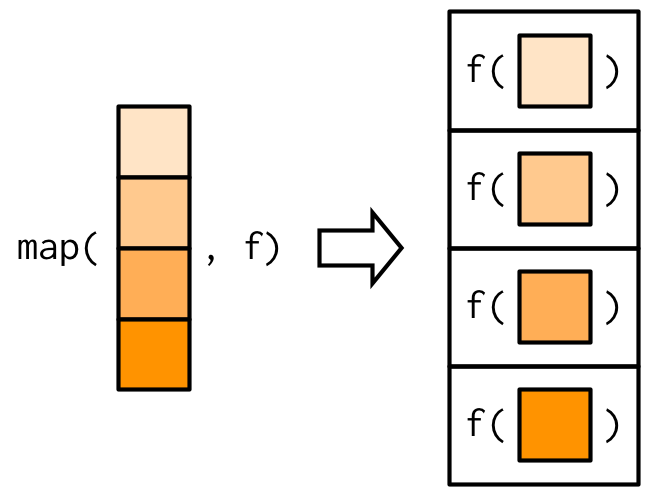
\includegraphics[width=9.01in]{../img/map_advr} \end{center}
\end{frame}

\begin{frame}[fragile]{Example 1}
\protect\hypertarget{example-1}{}
\begin{Shaded}
\begin{Highlighting}[]
\NormalTok{sheets }\OtherTok{\textless{}{-}} \FunctionTok{c}\NormalTok{( }\StringTok{"(NAP)全国"}\NormalTok{,}
        \StringTok{"(NAP)関西"}\NormalTok{,}
        \StringTok{"(NAP)関西以外"}\NormalTok{)}

\NormalTok{poo }\OtherTok{\textless{}{-}} \FunctionTok{map}\NormalTok{(sheets,}
\NormalTok{       read\_excel,}
       \AttributeTok{path =} \StringTok{"input/★【weekly】POO\_Flex\_Histrical\_Data.xlsx"}\NormalTok{,}
       \AttributeTok{trim\_ws =}\NormalTok{ F)}
\end{Highlighting}
\end{Shaded}
\end{frame}

\begin{frame}[fragile]{\texttt{map}一族}
\protect\hypertarget{mapux4e00ux65cf}{}
戻り値をリストではない形式に変換して返すこともできる

\begin{itemize}
\tightlist
\item
  \texttt{map} makes a list.
\item
  \texttt{map\_lgl} makes a logical vector.
\item
  \texttt{map\_int} makes an integer vector.
\item
  \texttt{map\_dbl} makes a double vector.
\item
  \texttt{map\_chr} makes a character vector.
\item
  \texttt{map\_df} makes a dataframe \textbf{特に重要}
\end{itemize}

これらが使えるかは\texttt{.f}の戻り値しだい
\end{frame}

\begin{frame}[fragile]{Example 2}
\protect\hypertarget{example-2}{}
\begin{Shaded}
\begin{Highlighting}[]
\NormalTok{sheets }\OtherTok{\textless{}{-}} \FunctionTok{c}\NormalTok{( }\StringTok{"(NAP)全国"}\NormalTok{,}
        \StringTok{"(NAP)関西"}\NormalTok{,}
        \StringTok{"(NAP)関西以外"}\NormalTok{)}

\NormalTok{poo }\OtherTok{\textless{}{-}} \FunctionTok{map\_df}\NormalTok{(sheets,}
\NormalTok{       read\_excel,}
       \AttributeTok{path =} \StringTok{"input/★【weekly】POO\_Flex\_Histrical\_Data.xlsx"}\NormalTok{,}
       \AttributeTok{trim\_ws =}\NormalTok{ F)}
\end{Highlighting}
\end{Shaded}
\end{frame}

\begin{frame}{\texttt{map}でやると何がいいのか}
\protect\hypertarget{mapux3067ux3084ux308bux3068ux4f55ux304cux3044ux3044ux306eux304b}{}
\begin{itemize}
\tightlist
\item
  読みやすい、書きやすい

  \begin{itemize}
  \tightlist
  \item
    ループは本来処理したいことに対して余計なモノが多すぎる
  \end{itemize}
\item
  処理が早い

  \begin{itemize}
  \tightlist
  \item
    と昔は言われていたが今はそうでもないらしい
  \item
    内部的にはCで処理しているから少し早い
  \end{itemize}
\end{itemize}
\end{frame}

\begin{frame}[fragile]{21.5.1 Shortcuts}
\protect\hypertarget{shortcuts}{}
\texttt{map}を使う上でのテクニック
\end{frame}

\begin{frame}[fragile]{余裕のあるやり方}
\protect\hypertarget{ux4f59ux88d5ux306eux3042ux308bux3084ux308aux65b9}{}
関数を定義する

\begin{Shaded}
\begin{Highlighting}[]
\NormalTok{mylm }\OtherTok{\textless{}{-}} \ControlFlowTok{function}\NormalTok{(df)\{}
  \FunctionTok{lm}\NormalTok{(mpg }\SpecialCharTok{\textasciitilde{}}\NormalTok{ wt, }\AttributeTok{data =}\NormalTok{ df)}
\NormalTok{\}}
\NormalTok{models }\OtherTok{\textless{}{-}}\NormalTok{ mtcars }\SpecialCharTok{\%\textgreater{}\%}
  \FunctionTok{split}\NormalTok{(.}\SpecialCharTok{$}\NormalTok{cyl) }\SpecialCharTok{\%\textgreater{}\%}
  \FunctionTok{map}\NormalTok{(mylm)}
\end{Highlighting}
\end{Shaded}
\end{frame}

\begin{frame}[fragile]{せっかちなやり方}
\protect\hypertarget{ux305bux3063ux304bux3061ux306aux3084ux308aux65b9}{}
\begin{block}{無名関数}
\protect\hypertarget{ux7121ux540dux95a2ux6570}{}
\begin{Shaded}
\begin{Highlighting}[]
\NormalTok{models }\OtherTok{\textless{}{-}}\NormalTok{ mtcars }\SpecialCharTok{\%\textgreater{}\%}
  \FunctionTok{split}\NormalTok{(.}\SpecialCharTok{$}\NormalTok{cyl) }\SpecialCharTok{\%\textgreater{}\%}
  \FunctionTok{map}\NormalTok{(}\ControlFlowTok{function}\NormalTok{(df)}\FunctionTok{lm}\NormalTok{(mpg }\SpecialCharTok{\textasciitilde{}}\NormalTok{ wt, }\AttributeTok{data =}\NormalTok{ df))}
\end{Highlighting}
\end{Shaded}
\end{block}

\begin{block}{formula}
\protect\hypertarget{formula}{}
\begin{Shaded}
\begin{Highlighting}[]
\NormalTok{models }\OtherTok{\textless{}{-}}\NormalTok{ mtcars }\SpecialCharTok{\%\textgreater{}\%}
  \FunctionTok{split}\NormalTok{(.}\SpecialCharTok{$}\NormalTok{cyl) }\SpecialCharTok{\%\textgreater{}\%}
  \FunctionTok{map}\NormalTok{(}\SpecialCharTok{\textasciitilde{}}\FunctionTok{lm}\NormalTok{(mpg }\SpecialCharTok{\textasciitilde{}}\NormalTok{ wt, }\AttributeTok{data =}\NormalTok{ .))}
\end{Highlighting}
\end{Shaded}
\end{block}
\end{frame}

\begin{frame}[fragile]{Example 3}
\protect\hypertarget{example-3}{}
\begin{Shaded}
\begin{Highlighting}[]
\NormalTok{sheets }\OtherTok{\textless{}{-}} \FunctionTok{c}\NormalTok{( }\StringTok{"(NAP)全国"}\NormalTok{,}
        \StringTok{"(NAP)関西"}\NormalTok{,}
        \StringTok{"(NAP)関西以外"}\NormalTok{)}

\NormalTok{poo }\OtherTok{\textless{}{-}} \FunctionTok{map\_df}\NormalTok{(sheets,}
       \SpecialCharTok{\textasciitilde{}}\FunctionTok{read\_excel}\NormalTok{(}
         \AttributeTok{sheet =}\NormalTok{ .,}
         \AttributeTok{path =} \StringTok{"input/★【weekly】POO\_Flex\_Histrical\_Data.xlsx"}\NormalTok{,}
         \AttributeTok{trim\_ws =} \ConstantTok{FALSE}
\NormalTok{       ) }\SpecialCharTok{\%\textgreater{}\%} 
         \FunctionTok{mutate}\NormalTok{(}\AttributeTok{sheet\_name =}\NormalTok{ .)}
\NormalTok{     ) }
\end{Highlighting}
\end{Shaded}
\end{frame}

\begin{frame}[fragile]{リストの各要素から情報を取り出す}
\protect\hypertarget{ux30eaux30b9ux30c8ux306eux5404ux8981ux7d20ux304bux3089ux60c5ux5831ux3092ux53d6ux308aux51faux3059}{}
\begin{Shaded}
\begin{Highlighting}[]
\NormalTok{models }\SpecialCharTok{\%\textgreater{}\%} 
  \FunctionTok{map}\NormalTok{(summary) }\SpecialCharTok{\%\textgreater{}\%} 
  \FunctionTok{map\_dbl}\NormalTok{(}\SpecialCharTok{\textasciitilde{}}\NormalTok{.}\SpecialCharTok{$}\NormalTok{r.squared)}
\end{Highlighting}
\end{Shaded}

\begin{verbatim}
##         4         6         8 
## 0.5086326 0.4645102 0.4229655
\end{verbatim}

\begin{block}{shortcut}
\protect\hypertarget{shortcut}{}
\begin{Shaded}
\begin{Highlighting}[]
\NormalTok{models }\SpecialCharTok{\%\textgreater{}\%}
  \FunctionTok{map}\NormalTok{(summary) }\SpecialCharTok{\%\textgreater{}\%}
  \FunctionTok{map\_dbl}\NormalTok{(}\StringTok{"r.squared"}\NormalTok{)}
\end{Highlighting}
\end{Shaded}
\end{block}
\end{frame}

\begin{frame}[fragile]{21.5.2 BaseR}
\protect\hypertarget{baser}{}
\texttt{lapply}, \texttt{sapply},
\texttt{vapply}という関数がbaseにある。

\texttt{map}を学べば不要
\end{frame}

\begin{frame}{21.5.3 Exercises}
\protect\hypertarget{exercises-3}{}
全部自分でやらなければ身につかない
\end{frame}

\begin{frame}[fragile]{21.6 Dealing with failure}
\protect\hypertarget{dealing-with-failure}{}
\texttt{map}関数を使ったプログラムのデバッグ技術

\texttt{map}中に一つエラーがあると全部出力しなくてむかつく

\begin{block}{for programmer}
\protect\hypertarget{for-programmer}{}
例外処理
\end{block}
\end{frame}

\begin{frame}[fragile]{\texttt{purrr::safely}}
\protect\hypertarget{purrrsafely}{}
関数\texttt{safely}は関数\texttt{.f}を引数として、\texttt{.f}を修正した関数を返す。

修正された関数は必ず長さ2のリストを返す関数で、その戻り値は下記の通り

\begin{enumerate}
\tightlist
\item
  要素\texttt{result}は元々の関数\texttt{.f}の結果。ただしその結果がエラーだった場合は\texttt{NULL}
\item
  要素\texttt{error}はエラーオブジェクト。\texttt{.f}の結果がエラーでなければ\texttt{NULL}
\end{enumerate}
\end{frame}

\begin{frame}[fragile]{Example 1}
\protect\hypertarget{example-1-1}{}
\begin{Shaded}
\begin{Highlighting}[]
\NormalTok{safe\_log }\OtherTok{\textless{}{-}} \FunctionTok{safely}\NormalTok{(log)}
\FunctionTok{safe\_log}\NormalTok{(}\DecValTok{10}\NormalTok{)}
\end{Highlighting}
\end{Shaded}

\begin{verbatim}
## $result
## [1] 2.302585
## 
## $error
## NULL
\end{verbatim}

\begin{Shaded}
\begin{Highlighting}[]
\FunctionTok{safe\_log}\NormalTok{(}\StringTok{"a"}\NormalTok{)}
\end{Highlighting}
\end{Shaded}

\begin{verbatim}
## $result
## NULL
## 
## $error
## <simpleError in .Primitive("log")(x, base):  数学関数に数値でない引数が渡されました >
\end{verbatim}
\end{frame}

\begin{frame}[fragile]{Example 2}
\protect\hypertarget{example-2-1}{}
\begin{Shaded}
\begin{Highlighting}[]
\NormalTok{x }\OtherTok{\textless{}{-}} \FunctionTok{list}\NormalTok{(}\DecValTok{1}\NormalTok{, }\DecValTok{10}\NormalTok{, }\StringTok{"a"}\NormalTok{)}
\NormalTok{y }\OtherTok{\textless{}{-}}\NormalTok{ x }\SpecialCharTok{\%\textgreater{}\%} \FunctionTok{map}\NormalTok{(}\FunctionTok{safely}\NormalTok{(log))}
\FunctionTok{str}\NormalTok{(y)}
\end{Highlighting}
\end{Shaded}

\begin{verbatim}
## List of 3
##  $ :List of 2
##   ..$ result: num 0
##   ..$ error : NULL
##  $ :List of 2
##   ..$ result: num 2.3
##   ..$ error : NULL
##  $ :List of 2
##   ..$ result: NULL
##   ..$ error :List of 2
##   .. ..$ message: chr " 数学関数に数値でない引数が渡されました "
##   .. ..$ call   : language .Primitive("log")(x, base)
##   .. ..- attr(*, "class")= chr [1:3] "simpleError" "error" "condition"
\end{verbatim}
\end{frame}

\begin{frame}[fragile]{\texttt{purrr::transpose}}
\protect\hypertarget{purrrtranspose}{}
関数\texttt{transpose}でもっと見易く

\begin{Shaded}
\begin{Highlighting}[]
\NormalTok{y }\OtherTok{\textless{}{-}}\NormalTok{ y }\SpecialCharTok{\%\textgreater{}\%}\NormalTok{ transpose}
\FunctionTok{str}\NormalTok{(y)}
\end{Highlighting}
\end{Shaded}

\begin{verbatim}
## List of 2
##  $ result:List of 3
##   ..$ : num 0
##   ..$ : num 2.3
##   ..$ : NULL
##  $ error :List of 3
##   ..$ : NULL
##   ..$ : NULL
##   ..$ :List of 2
##   .. ..$ message: chr " 数学関数に数値でない引数が渡されました "
##   .. ..$ call   : language .Primitive("log")(x, base)
##   .. ..- attr(*, "class")= chr [1:3] "simpleError" "error" "condition"
\end{verbatim}
\end{frame}

\begin{frame}[fragile]{一族 \texttt{purrr::possibly}}
\protect\hypertarget{ux4e00ux65cf-purrrpossibly}{}
関数\texttt{.f}がエラーのときに返す値を第二引数に指定できる。

\begin{Shaded}
\begin{Highlighting}[]
\NormalTok{possibly\_log }\OtherTok{\textless{}{-}} \FunctionTok{possibly}\NormalTok{(log, }\ConstantTok{NA}\NormalTok{)}
\FunctionTok{possibly\_log}\NormalTok{(}\DecValTok{10}\NormalTok{)}
\end{Highlighting}
\end{Shaded}

\begin{verbatim}
## [1] 2.302585
\end{verbatim}

\begin{Shaded}
\begin{Highlighting}[]
\FunctionTok{possibly\_log}\NormalTok{(}\StringTok{"a"}\NormalTok{)}
\end{Highlighting}
\end{Shaded}

\begin{verbatim}
## [1] NA
\end{verbatim}

全くエラーを返さなくなる
\end{frame}

\begin{frame}[fragile]{21.7 Mapping over multiple arguments}
\protect\hypertarget{mapping-over-multiple-arguments}{}
複数入力の\texttt{map}
\end{frame}

\begin{frame}[fragile]{\texttt{purrr::map2}}
\protect\hypertarget{purrrmap2}{}
\begin{block}{Usage}
\protect\hypertarget{usage-1}{}
\begin{Shaded}
\begin{Highlighting}[]
\FunctionTok{map2}\NormalTok{(.x, .y, .f, ...)}
\end{Highlighting}
\end{Shaded}
\end{block}

\begin{block}{Arguments}
\protect\hypertarget{arguments-1}{}
\begin{longtable}[]{@{}
  >{\raggedright\arraybackslash}p{(\columnwidth - 2\tabcolsep) * \real{0.5000}}
  >{\raggedright\arraybackslash}p{(\columnwidth - 2\tabcolsep) * \real{0.5000}}@{}}
\toprule()
\endhead
\textbf{.x} & listかatomic vector \\
\textbf{.y} & listかatomic
vector。.xと.yとのそれぞれのベクトルの長さが同じでなければならない \\
\textbf{.f} & 関数かformula \\
\textbf{\ldots{}} &
関数に渡すパラメータ。たとえば\texttt{na.rm\ =\ TRUE} \\
\bottomrule()
\end{longtable}
\end{block}

\begin{block}{return}
\protect\hypertarget{return-1}{}
ベクトル\texttt{.x},\texttt{.y}の要素をそれぞれ関数\texttt{.f}に適用し、その結果をリストで返す
\end{block}
\end{frame}

\begin{frame}[fragile]{Example}
\protect\hypertarget{example}{}
\begin{Shaded}
\begin{Highlighting}[]
\NormalTok{mu }\OtherTok{\textless{}{-}} \FunctionTok{list}\NormalTok{(}\DecValTok{5}\NormalTok{, }\DecValTok{10}\NormalTok{, }\SpecialCharTok{{-}}\DecValTok{3}\NormalTok{)}
\NormalTok{sigma }\OtherTok{\textless{}{-}} \FunctionTok{list}\NormalTok{(}\DecValTok{1}\NormalTok{, }\DecValTok{5}\NormalTok{, }\DecValTok{10}\NormalTok{)}
\FunctionTok{map2}\NormalTok{(mu, sigma, rnorm, }\AttributeTok{n =} \DecValTok{5}\NormalTok{)}
\end{Highlighting}
\end{Shaded}

\begin{verbatim}
## [[1]]
## [1] 4.406548 3.787894 5.002558 4.143748 4.264373
## 
## [[2]]
## [1]  9.009236  9.457236  8.820623 14.652523 12.621634
## 
## [[3]]
## [1]   5.089128   3.706198 -13.411853   7.017456 -14.014834
\end{verbatim}
\end{frame}

\begin{frame}{Visualization of map2}
\protect\hypertarget{visualization-of-map2}{}
\begin{figure}
\centering
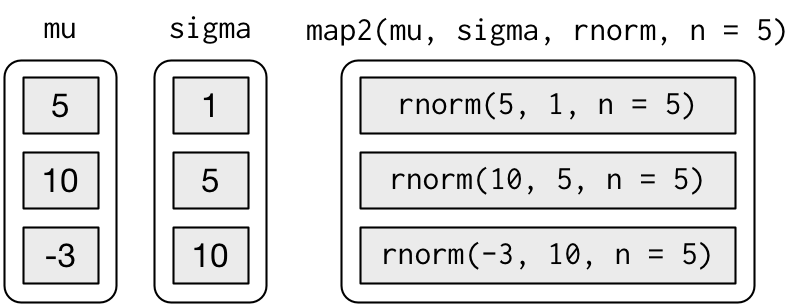
\includegraphics{../img/lists-map2.png}
\caption{structure of map2}
\end{figure}
\end{frame}

\begin{frame}[fragile]{\texttt{purrr::pmap}}
\protect\hypertarget{purrrpmap}{}
入力が3つ以上の場合

\begin{Shaded}
\begin{Highlighting}[]
\NormalTok{n }\OtherTok{\textless{}{-}} \FunctionTok{list}\NormalTok{(}\DecValTok{1}\NormalTok{, }\DecValTok{3}\NormalTok{, }\DecValTok{5}\NormalTok{)}
\NormalTok{args2 }\OtherTok{\textless{}{-}} \FunctionTok{list}\NormalTok{(}\AttributeTok{mean =}\NormalTok{ mu, }\AttributeTok{sd =}\NormalTok{ sigma, }\AttributeTok{n =}\NormalTok{ n)}
\NormalTok{args2 }\SpecialCharTok{\%\textgreater{}\%} \FunctionTok{pmap}\NormalTok{(rnorm) }\SpecialCharTok{\%\textgreater{}\%} \FunctionTok{str}\NormalTok{()}
\end{Highlighting}
\end{Shaded}

\begin{verbatim}
## List of 3
##  $ : num 5.45
##  $ : num [1:3] 13.8 18.2 15.3
##  $ : num [1:5] -3.02 -5.15 -23.11 -13.03 -2.59
\end{verbatim}
\end{frame}

\begin{frame}{Visualization of pmap}
\protect\hypertarget{visualization-of-pmap}{}
\begin{figure}
\centering
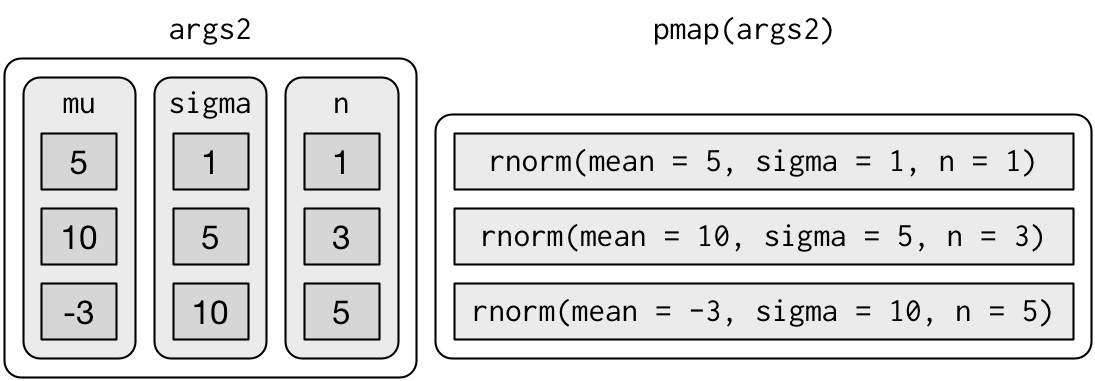
\includegraphics{../img/lists-pmap-named.png}
\caption{structure of pmap}
\end{figure}
\end{frame}

\begin{frame}[fragile]{これでもいいよ}
\protect\hypertarget{ux3053ux308cux3067ux3082ux3044ux3044ux3088}{}
\begin{Shaded}
\begin{Highlighting}[]
\NormalTok{params }\OtherTok{\textless{}{-}} \FunctionTok{tribble}\NormalTok{(}
          \SpecialCharTok{\textasciitilde{}}\NormalTok{mean, }\SpecialCharTok{\textasciitilde{}}\NormalTok{sd, }\SpecialCharTok{\textasciitilde{}}\NormalTok{n,}
          \DecValTok{5}\NormalTok{,     }\DecValTok{1}\NormalTok{,   }\DecValTok{1}\NormalTok{,}
          \DecValTok{10}\NormalTok{,    }\DecValTok{5}\NormalTok{,   }\DecValTok{3}\NormalTok{,}
          \SpecialCharTok{{-}}\DecValTok{3}\NormalTok{,    }\DecValTok{10}\NormalTok{,  }\DecValTok{5}\NormalTok{)}
\NormalTok{params }\SpecialCharTok{\%\textgreater{}\%} \FunctionTok{pmap}\NormalTok{(rnorm)}
\end{Highlighting}
\end{Shaded}

\begin{verbatim}
## [[1]]
## [1] 5.027279
## 
## [[2]]
## [1] 7.741559 9.245711 6.816939
## 
## [[3]]
## [1]  5.370907 -9.774716 -1.475768  5.704987 -4.147142
\end{verbatim}
\end{frame}

\begin{frame}[fragile]{21.7.1 Involing different functions}
\protect\hypertarget{involing-different-functions}{}
入力変数だけでなく処理する関数すら変えたい場合

\begin{block}{Notes!!}
\protect\hypertarget{notes}{}
現在\texttt{invoke\_map}は非推奨になっている。\texttt{exec}で代用するべしとある
\end{block}
\end{frame}

\begin{frame}[fragile]{\texttt{invoke\_map}}
\protect\hypertarget{invoke_map}{}
関数名を文字列でわたす

\begin{Shaded}
\begin{Highlighting}[]
\NormalTok{f }\OtherTok{\textless{}{-}} \FunctionTok{c}\NormalTok{(}\StringTok{"runif"}\NormalTok{, }\StringTok{"rnorm"}\NormalTok{, }\StringTok{"rpois"}\NormalTok{)}
\NormalTok{param }\OtherTok{\textless{}{-}} \FunctionTok{list}\NormalTok{(}
          \FunctionTok{list}\NormalTok{(}\AttributeTok{min =} \SpecialCharTok{{-}}\DecValTok{1}\NormalTok{, }\AttributeTok{max =} \DecValTok{1}\NormalTok{), }
          \FunctionTok{list}\NormalTok{(}\AttributeTok{sd =} \DecValTok{5}\NormalTok{), }
          \FunctionTok{list}\NormalTok{(}\AttributeTok{lambda =} \DecValTok{10}\NormalTok{))}
\FunctionTok{invoke\_map}\NormalTok{(f, param, }\AttributeTok{n =} \DecValTok{5}\NormalTok{)}
\end{Highlighting}
\end{Shaded}

\begin{verbatim}
## [[1]]
## [1]  0.91406237 -0.48443496  0.68515139 -0.03189625  0.45374870
## 
## [[2]]
## [1] -7.78456256  4.06060522  5.02826919 -0.05041309  1.03358154
## 
## [[3]]
## [1] 18 10 11  6 14
\end{verbatim}
\end{frame}

\begin{frame}{Visualization of \texttt{invoke\_map}}
\protect\hypertarget{visualization-of-invoke_map}{}
\begin{figure}
\centering
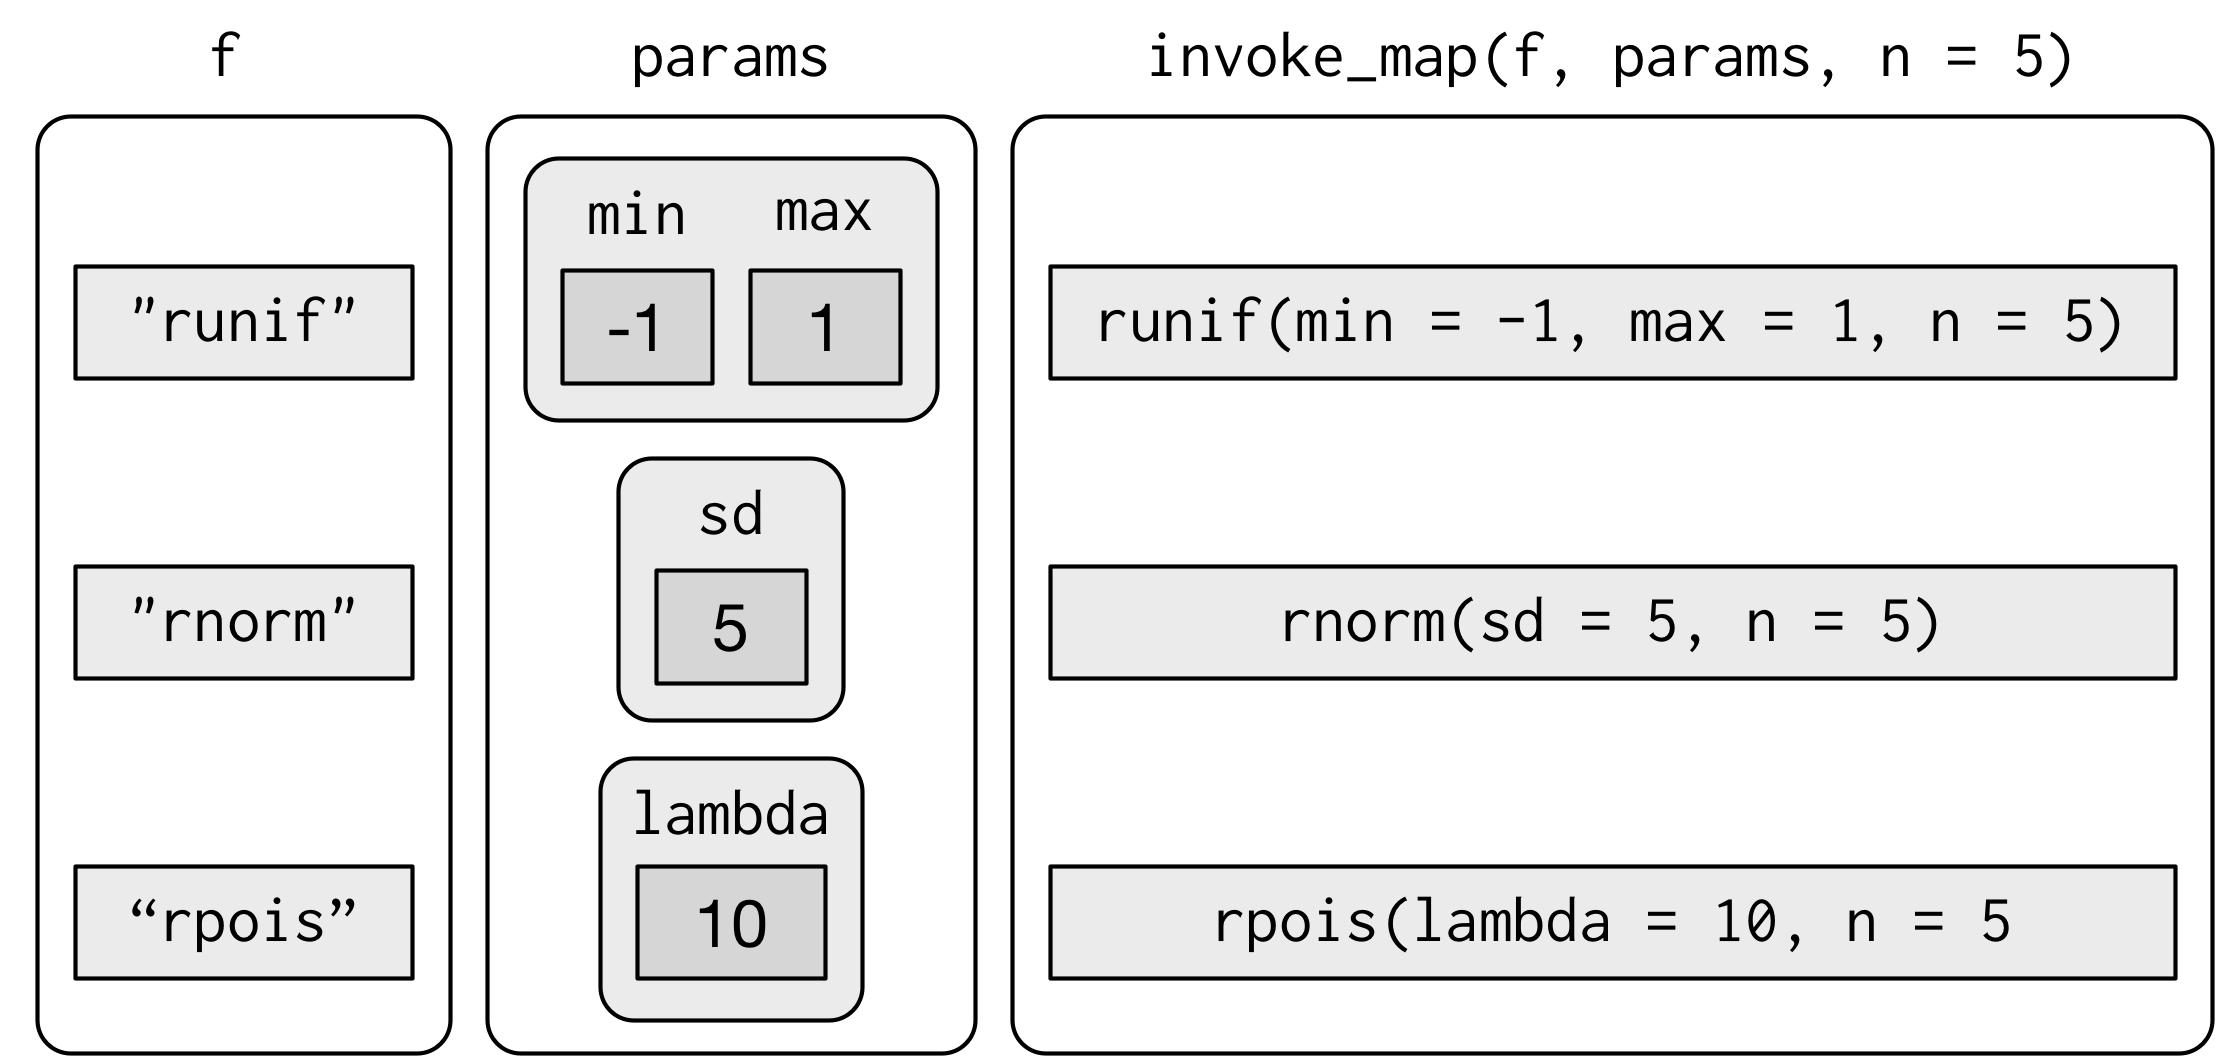
\includegraphics{../img/lists-invoke.png}
\caption{structure of invoke}
\end{figure}
\end{frame}

\begin{frame}[fragile]{\texttt{exec}で置き換え}
\protect\hypertarget{execux3067ux7f6eux304dux63dbux3048}{}
\begin{Shaded}
\begin{Highlighting}[]
\CommentTok{\# Before:}
\FunctionTok{invoke\_map}\NormalTok{(fns, }\FunctionTok{list}\NormalTok{(args))}
\FunctionTok{invoke\_map}\NormalTok{(fns, }\FunctionTok{list}\NormalTok{(args1, args2))}

\CommentTok{\# After:}
\FunctionTok{map}\NormalTok{(fns, exec, }\SpecialCharTok{!!!}\NormalTok{args)}
\FunctionTok{map2}\NormalTok{(fns, }\FunctionTok{list}\NormalTok{(args1, args2), }\ControlFlowTok{function}\NormalTok{(fn, args) }\FunctionTok{exec}\NormalTok{(fn, }\SpecialCharTok{!!!}\NormalTok{args))}
\end{Highlighting}
\end{Shaded}

\url{https://github.com/tidyverse/purrr/blob/master/NEWS.md\#retirement-of-invoke}
\end{frame}

\begin{frame}{21.8 Walk}
\protect\hypertarget{walk}{}
副作用を目的にFPを
\end{frame}

\begin{frame}[fragile]{\texttt{purrr::walk}}
\protect\hypertarget{purrrwalk}{}
\begin{Shaded}
\begin{Highlighting}[]
\NormalTok{x }\OtherTok{\textless{}{-}} \FunctionTok{list}\NormalTok{(}\DecValTok{1}\NormalTok{, }\StringTok{"a"}\NormalTok{, }\DecValTok{3}\NormalTok{) }

\NormalTok{x }\SpecialCharTok{\%\textgreater{}\%} \FunctionTok{walk}\NormalTok{(print)}
\end{Highlighting}
\end{Shaded}

\begin{verbatim}
## [1] 1
## [1] "a"
## [1] 3
\end{verbatim}
\end{frame}

\begin{frame}[fragile]{\texttt{purrr::pwalk}}
\protect\hypertarget{purrrpwalk}{}
\begin{Shaded}
\begin{Highlighting}[]
\NormalTok{plots }\OtherTok{\textless{}{-}}\NormalTok{ mtcars }\SpecialCharTok{\%\textgreater{}\%} 
  \FunctionTok{split}\NormalTok{(.}\SpecialCharTok{$}\NormalTok{cyl) }\SpecialCharTok{\%\textgreater{}\%} 
  \FunctionTok{map}\NormalTok{(}\SpecialCharTok{\textasciitilde{}}\FunctionTok{ggplot}\NormalTok{(., }\FunctionTok{aes}\NormalTok{(mpg, wt)) }\SpecialCharTok{+} \FunctionTok{geom\_point}\NormalTok{())}
\NormalTok{paths }\OtherTok{\textless{}{-}}\NormalTok{ stringr}\SpecialCharTok{::}\FunctionTok{str\_c}\NormalTok{(}\FunctionTok{names}\NormalTok{(plots), }\StringTok{".pdf"}\NormalTok{) }
\FunctionTok{pwalk}\NormalTok{(}\FunctionTok{list}\NormalTok{(paths, plots), ggsave, }\AttributeTok{path =} \FunctionTok{tempdir}\NormalTok{())}
\end{Highlighting}
\end{Shaded}
\end{frame}

\begin{frame}[fragile]{21.9 Other patterns of for loops}
\protect\hypertarget{other-patterns-of-for-loops}{}
FPのバリエーション

\texttt{map}ほどは使わないが頭のどこかに置いておくといいことがあるかもしれない
\end{frame}

\begin{frame}{21.9.1 Predicate functions}
\protect\hypertarget{predicate-functions}{}
入力関数として出力が論理値の関数を受け付けて特殊な動作をする
\end{frame}

\begin{frame}[fragile]{\texttt{purrr::keep}と\texttt{purrr::discard}}
\protect\hypertarget{purrrkeepux3068purrrdiscard}{}
入力ベクトルの要素のうち、関数の判定が\texttt{TRUE}の要素のみを残す(捨てる)

入力がデータフレームなら\texttt{dplyr::select\_if}と同じ

\begin{Shaded}
\begin{Highlighting}[]
\NormalTok{iris }\SpecialCharTok{\%\textgreater{}\%} \FunctionTok{keep}\NormalTok{(is.factor) }\SpecialCharTok{\%\textgreater{}\%}\NormalTok{ str}
\end{Highlighting}
\end{Shaded}

\begin{verbatim}
## 'data.frame':    150 obs. of  1 variable:
##  $ Species: Factor w/ 3 levels "setosa","versicolor",..: 1 1 1 1 1 1 1 1 1 1 ...
\end{verbatim}

\begin{Shaded}
\begin{Highlighting}[]
\NormalTok{iris }\SpecialCharTok{\%\textgreater{}\%} \FunctionTok{discard}\NormalTok{(is.factor) }\SpecialCharTok{\%\textgreater{}\%}\NormalTok{ str}
\end{Highlighting}
\end{Shaded}

\begin{verbatim}
## 'data.frame':    150 obs. of  4 variables:
##  $ Sepal.Length: num  5.1 4.9 4.7 4.6 5 5.4 4.6 5 4.4 4.9 ...
##  $ Sepal.Width : num  3.5 3 3.2 3.1 3.6 3.9 3.4 3.4 2.9 3.1 ...
##  $ Petal.Length: num  1.4 1.4 1.3 1.5 1.4 1.7 1.4 1.5 1.4 1.5 ...
##  $ Petal.Width : num  0.2 0.2 0.2 0.2 0.2 0.4 0.3 0.2 0.2 0.1 ...
\end{verbatim}
\end{frame}

\begin{frame}[fragile]{\texttt{purrr::some}と\texttt{purrr::every}}
\protect\hypertarget{purrrsomeux3068purrrevery}{}
入力ベクトルの要素のうち、関数の判定がどれか(すべて)が\texttt{TRUE}なら\texttt{TRUE}

\begin{Shaded}
\begin{Highlighting}[]
\NormalTok{x }\OtherTok{\textless{}{-}} \FunctionTok{list}\NormalTok{(}\DecValTok{1}\SpecialCharTok{:}\DecValTok{5}\NormalTok{, letters, }\FunctionTok{list}\NormalTok{(}\DecValTok{10}\NormalTok{))}

\NormalTok{x }\SpecialCharTok{\%\textgreater{}\%} \FunctionTok{some}\NormalTok{(is\_character)}
\end{Highlighting}
\end{Shaded}

\begin{verbatim}
## [1] TRUE
\end{verbatim}

\begin{Shaded}
\begin{Highlighting}[]
\NormalTok{x }\SpecialCharTok{\%\textgreater{}\%} \FunctionTok{every}\NormalTok{(is\_vector)}
\end{Highlighting}
\end{Shaded}

\begin{verbatim}
## [1] TRUE
\end{verbatim}
\end{frame}

\begin{frame}[fragile]{\texttt{purrr::detect}}
\protect\hypertarget{purrrdetect}{}
条件が成立する最初の要素の値を返す。

\begin{Shaded}
\begin{Highlighting}[]
\NormalTok{x }\OtherTok{\textless{}{-}} \FunctionTok{sample}\NormalTok{(}\DecValTok{10}\NormalTok{)}
\NormalTok{x}
\end{Highlighting}
\end{Shaded}

\begin{verbatim}
##  [1]  2  4  6  1  5  3  7 10  9  8
\end{verbatim}

\begin{Shaded}
\begin{Highlighting}[]
\NormalTok{x }\SpecialCharTok{\%\textgreater{}\%} \FunctionTok{detect}\NormalTok{(}\SpecialCharTok{\textasciitilde{}}\NormalTok{ . }\SpecialCharTok{\textgreater{}} \DecValTok{5}\NormalTok{)}
\end{Highlighting}
\end{Shaded}

\begin{verbatim}
## [1] 6
\end{verbatim}

\begin{Shaded}
\begin{Highlighting}[]
\NormalTok{x }\SpecialCharTok{\%\textgreater{}\%} \FunctionTok{detect\_index}\NormalTok{(}\SpecialCharTok{\textasciitilde{}}\NormalTok{ . }\SpecialCharTok{\textgreater{}} \DecValTok{5}\NormalTok{)}
\end{Highlighting}
\end{Shaded}

\begin{verbatim}
## [1] 3
\end{verbatim}
\end{frame}

\begin{frame}[fragile]{\texttt{purrr::head\_while}と\texttt{purrr::tail\_while}}
\protect\hypertarget{purrrhead_whileux3068purrrtail_while}{}
条件が成り立つまでの要素をすべて返す。

前から調べるか、後ろから調べるか

\begin{Shaded}
\begin{Highlighting}[]
\NormalTok{x }\SpecialCharTok{\%\textgreater{}\%} \FunctionTok{head\_while}\NormalTok{(}\SpecialCharTok{\textasciitilde{}}\NormalTok{ . }\SpecialCharTok{\textgreater{}} \DecValTok{5}\NormalTok{)}
\end{Highlighting}
\end{Shaded}

\begin{verbatim}
## integer(0)
\end{verbatim}

\begin{Shaded}
\begin{Highlighting}[]
\NormalTok{x }\SpecialCharTok{\%\textgreater{}\%} \FunctionTok{tail\_while}\NormalTok{(}\SpecialCharTok{\textasciitilde{}}\NormalTok{ . }\SpecialCharTok{\textgreater{}} \DecValTok{5}\NormalTok{)}
\end{Highlighting}
\end{Shaded}

\begin{verbatim}
## [1]  7 10  9  8
\end{verbatim}
\end{frame}

\begin{frame}{21.9.2 Reduce and accumulate}
\protect\hypertarget{reduce-and-accumulate}{}
2入力1出力関数のみを受け付ける特殊な関数

2つの入力の順序を入れ替えても出力の値が変わらない場合が望ましい
\end{frame}

\begin{frame}[fragile]{\texttt{purrr::reduce}}
\protect\hypertarget{purrrreduce}{}
\begin{Shaded}
\begin{Highlighting}[]
\NormalTok{dfs }\OtherTok{\textless{}{-}} \FunctionTok{list}\NormalTok{( }\AttributeTok{age =} \FunctionTok{tibble}\NormalTok{(}\AttributeTok{name =} \StringTok{"John"}\NormalTok{, }\AttributeTok{age =} \DecValTok{30}\NormalTok{),}
        \AttributeTok{sex =} \FunctionTok{tibble}\NormalTok{(}\AttributeTok{name =} \FunctionTok{c}\NormalTok{(}\StringTok{"John"}\NormalTok{, }\StringTok{"Mary"}\NormalTok{), }\AttributeTok{sex =} \FunctionTok{c}\NormalTok{(}\StringTok{"M"}\NormalTok{, }\StringTok{"F"}\NormalTok{)),}
        \AttributeTok{trt =} \FunctionTok{tibble}\NormalTok{(}\AttributeTok{name =} \StringTok{"Mary"}\NormalTok{, }\AttributeTok{treatment =} \StringTok{"A"}\NormalTok{))}
\NormalTok{dfs }\SpecialCharTok{\%\textgreater{}\%} \FunctionTok{reduce}\NormalTok{(full\_join)}
\end{Highlighting}
\end{Shaded}

\begin{verbatim}
## Joining, by = "name"
## Joining, by = "name"
\end{verbatim}

\begin{verbatim}
## # A tibble: 2 x 4
##   name    age sex   treatment
##   <chr> <dbl> <chr> <chr>    
## 1 John     30 M     <NA>     
## 2 Mary     NA F     A
\end{verbatim}
\end{frame}

\begin{frame}[fragile]{\texttt{purrr::accumulate}}
\protect\hypertarget{purrraccumulate}{}
\begin{Shaded}
\begin{Highlighting}[]
\NormalTok{x }\OtherTok{\textless{}{-}} \FunctionTok{sample}\NormalTok{(}\DecValTok{10}\NormalTok{)}
\NormalTok{x}
\end{Highlighting}
\end{Shaded}

\begin{verbatim}
##  [1]  2  1  7  4  9  6  3  8 10  5
\end{verbatim}

\begin{Shaded}
\begin{Highlighting}[]
\NormalTok{x }\SpecialCharTok{\%\textgreater{}\%} \FunctionTok{accumulate}\NormalTok{(}\StringTok{\textasciigrave{}}\AttributeTok{+}\StringTok{\textasciigrave{}}\NormalTok{)}
\end{Highlighting}
\end{Shaded}

\begin{verbatim}
##  [1]  2  3 10 14 23 29 32 40 50 55
\end{verbatim}
\end{frame}

\begin{frame}{21.9.3 Exercises}
\protect\hypertarget{exercises-4}{}
頭の訓練に
\end{frame}

\end{document}
